% ---------------------------------------------------------------------------
% Replaces \subsection{Subjective Evaluation (N-MOS)} and
% \subsection{Voice Turing Test}. About half a page each including the figure.
%
% Figures come from  python tools/make_paper_figures.py  (docs/paper/figures/).
% Numbers quoted in the prose are checked by tools/make_paper_tables.py.
% Source: evaluation/results/listening_test/*.csv, build 2026-09-10, seed 20260901.
% ---------------------------------------------------------------------------

\subsection{Subjective Evaluation (N-MOS)}
\label{subjective_evaluation}

Naturalness and prosody are not captured by the objective metrics and were
assessed in a listening test with $30$ native German speakers. Each rated
$24$ to $28$ excerpts on the five-point absolute category rating scale of
ITU-T P.800 (1 = bad, 5 = excellent), giving a naturalness mean opinion score
(N-MOS) \cite{xie2025controllablespeechsynthesisera}. The genuine recordings
were rated unlabelled among the clones. Two stimuli were repeated per rater
without announcement to measure rating consistency.

Stimuli are excerpts of about $10$\,s ($5.9$ to $14.4$\,s), cut on sentence
boundaries so that every condition presents the same passage of a text. All
stimuli, including the genuine recordings, passed through identical
processing: resampling to $24$\,kHz, loudness normalisation to $-23$\,LUFS
\cite{itu_bs1770} and a common pause noise floor. The last step is required
because the denoised recordings otherwise have digitally silent pauses that no
synthesis system produces, and a single threshold on that cue identified the
genuine recording in $96\,\%$ of stimuli before matching.

The score of a condition is the mean of per-rater means, so that every rater
carries equal weight. Confidence intervals come from a two-way cluster
bootstrap that resamples raters and texts, since neither answers of one rater
nor answers to one text are independent. Differences are paired within rater
and judged at a Bonferroni-adjusted level over six comparisons. A simulation of
this design before data collection gave a coverage of $0.99$ for the nominal
$95\,\%$ interval and $80\,\%$ power for a difference of $0.30$ MOS at $30$
raters, so smaller differences are reported as not detectable rather than as
absent.

\begin{figure}[H]
    \centering
    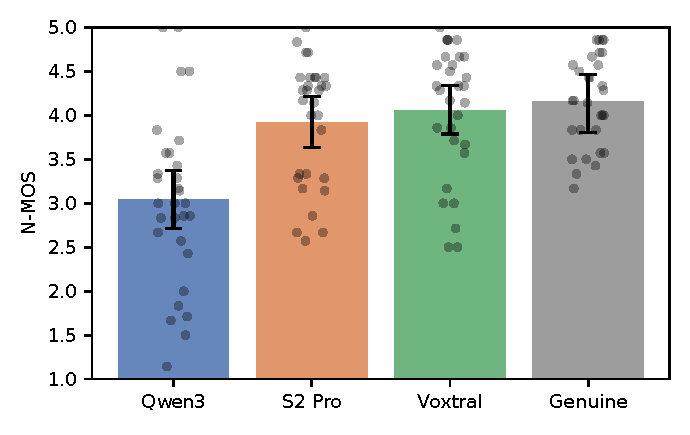
\includegraphics[width=0.62\linewidth]{figures/fig_nmos.pdf}
    \caption{Naturalness by condition. Bars are the mean of per-rater means
    with two-way cluster bootstrap $95\,\%$ intervals ($30$ raters, $13$
    texts); each dot is one rater's mean for that condition.}
    \label{fig:nmos}
\end{figure}

Figure~\ref{fig:nmos} shows the result. Qwen3 scores $3.04$ $[2.71, 3.37]$ and
lies $0.9$ to $1.1$ points below every other condition; all three differences
remain detectable after adjustment. S2 Pro ($3.92$ $[3.64, 4.22]$), Voxtral
($4.05$ $[3.79, 4.34]$) and the genuine recordings ($4.16$ $[3.81, 4.46]$) are
not distinguishable from each other: none of the three adjusted intervals
excludes zero. The rating noise sets the scale for these statements. Across
$60$ hidden repeats the mean absolute difference between two ratings of the
same stimulus by the same rater was $0.55$ points; the Qwen3 gap is well above
it, the gaps among the other three conditions ($0.10$ to $0.23$) are below it.

The ranking is the reverse of the similarity ranking in
Table~\ref{tab:objective_results}. The system whose clone is closest to the
patient by the speaker embedding is the one raters find least natural, and the
system with the lowest similarity is not distinguishable from the genuine
recordings. The preregistered hypothesis that naturalness follows similarity
is therefore rejected, and the finding is taken up in
Section~\ref{discussion}.

\subsection{Voice Turing Test}
\label{turing_test}

In the second part of the session each rater heard $6$ to $7$ pairs consisting
of the genuine recording and one clone of the same passage, and selected the
one they believed to be the patient. Order and sides were randomised, and no
rater met a text in both parts of the test. The fooling rate is the proportion
of pairs in which the clone was chosen; $0.50$ is chance and the best result a
clone can reach, values below it mean the clone was detected
\cite{xie2025controllablespeechsynthesisera}. $39$ pairs ($13$ per system) were
answered by $29$ raters, $15$ of whom know the patient personally.

\begin{figure}[H]
    \centering
    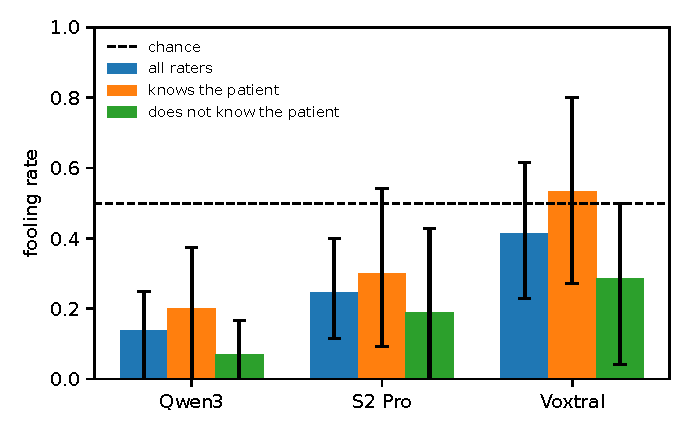
\includegraphics[width=0.62\linewidth]{figures/fig_turing.pdf}
    \caption{Fooling rate by system and rater group with two-way cluster
    bootstrap $95\,\%$ intervals. The dashed line is chance level.}
    \label{fig:turing}
\end{figure}

Detection differed sharply between systems (Figure~\ref{fig:turing}). Qwen3 was
identified most reliably ($0.14$ $[0.00, 0.25]$), followed by S2 Pro ($0.25$
$[0.12, 0.40]$); both lie below chance. Voxtral reached $0.41$ $[0.23, 0.62]$
and its interval includes $0.50$ in every rater group, so the preregistered
hypothesis that all three are detected above chance holds for two systems and
fails for Voxtral.

Raters who know the patient were fooled more often than strangers, for all three
systems, the opposite of the expected direction; for Voxtral this group chose
the clone in $0.53$ $[0.27, 0.80]$ of pairs. All three contrasts ($+0.13$,
$+0.11$, $+0.25$) have intervals containing zero, so at $15$ versus $14$ raters
this is a trend, not a result. The patient herself, kept out of all averages,
identified her own voice in $6$ of $6$ pairs.

The fooling rates are a lower bound. Pause structure, spectral brightness and
excerpt duration still separate genuine from cloned excerpts with paired
accuracies of $0.82$, $0.80$ and $0.72$ against chance $0.50$; they were left in
because pausing and timbre are part of what raters judge. The ordering
nevertheless reproduces the naturalness ranking, on disjoint texts and with a
different task, and both run counter to the similarity ranking in
Table~\ref{tab:objective_results}.
